\documentclass[10pt,a4paper]{article}
\usepackage[margin=1.4cm,top=1.1cm,bottom=1.0cm]{geometry}
\usepackage[T1]{fontenc}
\usepackage[utf8]{inputenc}
\usepackage{amsmath,amssymb}
\usepackage{xcolor}
\usepackage{framed}
\usepackage{tikz}
\usetikzlibrary{arrows.meta,backgrounds,calc}
\usepackage[hidelinks]{hyperref}
% Shared colours and boxes for tutorial.tex and cheatsheet.tex.
% Needs: xcolor, framed. (tcolorbox is not available in this TeX install.)

% ---------- palette ----------
\definecolor{secblue}{rgb}{0.10,0.22,0.48}
\definecolor{thmbg}{rgb}{0.93,0.95,1.00}   \definecolor{thmfr}{rgb}{0.20,0.33,0.68}
\definecolor{defbg}{rgb}{0.93,0.98,0.97}   \definecolor{deffr}{rgb}{0.05,0.45,0.42}
\definecolor{keybg}{rgb}{1.00,0.97,0.86}   \definecolor{keyfr}{rgb}{0.72,0.50,0.02}
\definecolor{recbg}{rgb}{0.94,0.96,0.98}   \definecolor{recfr}{rgb}{0.25,0.35,0.45}
\definecolor{clmbg}{rgb}{0.96,0.93,1.00}   \definecolor{clmfr}{rgb}{0.42,0.22,0.62}
\definecolor{ourbg}{rgb}{0.96,0.96,0.96}   \definecolor{ourfr}{rgb}{0.35,0.35,0.35}
\definecolor{okbg}{rgb}{0.92,0.98,0.92}    \definecolor{okfr}{rgb}{0.12,0.50,0.18}
\definecolor{nobg}{rgb}{1.00,0.93,0.92}    \definecolor{nofr}{rgb}{0.70,0.16,0.12}
\definecolor{codebg}{rgb}{0.965,0.965,0.955}
\definecolor{shadecolor}{rgb}{0.965,0.965,0.955}

% ---------- generic breakable colour box: \begin{cbox}[title]{background}{frame} ----------
\newenvironment{cbox}[3][]{%
  \def\FrameCommand{\fboxsep=7pt\fboxrule=0.9pt\fcolorbox{#3}{#2}}%
  \MakeFramed{\advance\hsize-\width\FrameRestore}%
  \if\relax\detokenize{#1}\relax\else
    {\noindent\textcolor{#3}{\sffamily\bfseries #1}\par\nobreak\vspace{3pt}}%
  \fi\noindent\ignorespaces}
 {\endMakeFramed}

% ---------- named boxes ----------
\newenvironment{keybox}[1][Key point]{\cbox[#1]{keybg}{keyfr}}{\endcbox}                 % take-aways
\newenvironment{recipebox}[1][Recipe]{\cbox[#1]{recbg}{recfr}}{\endcbox}                 % procedures
\newenvironment{claimbox}[1][Claims of the paper]{\cbox[#1]{clmbg}{clmfr}}{\endcbox}     % what a paper asks and claims
\newenvironment{oursbox}[1][Our reading]{\cbox[#1]{ourbg}{ourfr}}{\endcbox}              % remarks that are not the paper's
\newenvironment{okbox}[1][Guaranteed]{\cbox[#1]{okbg}{okfr}}{\endcbox}                   % what holds
\newenvironment{nobox}[1][Not guaranteed]{\cbox[#1]{nobg}{nofr}}{\endcbox}               % what does not
\newenvironment{thmbox}{\cbox{thmbg}{thmfr}}{\endcbox}
\newenvironment{defbox}{\cbox{defbg}{deffr}}{\endcbox}

% ---------- inline highlights ----------
\newcommand{\hl}[1]{\textcolor{secblue}{\textbf{#1}}}                    % key term
\newcommand{\yes}[1]{\textcolor{okfr}{\textbf{#1}}}
\newcommand{\no}[1]{\textcolor{nofr}{\textbf{#1}}}
\newcommand{\ctag}[1]{{\fboxsep=1.5pt\colorbox{clmfr}{\textcolor{white}{\sffamily\bfseries\scriptsize #1}}}}  % claim id
\newcommand{\kind}[1]{\textcolor{clmfr}{\textsf{\scriptsize[#1]}}}       % kind of claim


% ---------- notation ----------
\newcommand{\PP}{\mathbb{P}}
\newcommand{\Dtr}{D_{\rm train}}
\newcommand{\Dcal}{D_{\rm cal}}
\newcommand{\Bcal}{B_{\rm cal}}
\newcommand{\Bpred}{B_{\rm pred}}
\newcommand{\ths}{\theta^\star}
\newcommand{\tauhat}{\hat\tau}

% ---------- line badges: the same number marks a line in the figure, the algorithm and the text ----------
\tikzset{badge/.style={circle,fill=recfr,text=white,inner sep=0.6pt,minimum size=9pt,font=\sffamily\bfseries\fontsize{6}{6}\selectfont}}
\newcommand{\lb}[1]{\tikz[baseline=(b.base)]\node[badge](b){#1};}

% ---------- pseudocode: one \al per line, optional argument = indent in em ----------
\newcounter{algline}
\newenvironment{algo}{\begin{list}{}{\setlength{\leftmargin}{1.7em}\setlength{\labelwidth}{1.2em}\setlength{\labelsep}{0.5em}%
  \setlength{\itemsep}{2pt}\setlength{\parsep}{0pt}\setlength{\topsep}{2pt}\setlength{\partopsep}{0pt}}}{\end{list}}
\newcommand{\al}[1][0]{\stepcounter{algline}\item[\lb{\arabic{algline}}]\hspace*{#1em}\ignorespaces}
\newcommand{\kw}[1]{\textbf{#1}}
\newcommand{\cm}[1]{\hfill\textcolor{ourfr}{\scriptsize\itshape #1}}
\newcommand{\algin}[1]{\noindent\textcolor{recfr}{\textbf{Input:}} #1\par}

% ---------- claim cells for the figure ----------
\newcommand{\clm}[3]{{\fboxsep=1.3pt\fboxrule=0.4pt\fcolorbox{#1}{#2}{\tiny\strut$c_{#3}$}}}
\newcommand{\cany}[1]{\clm{recfr}{white}{#1}}
\newcommand{\ckeep}[1]{\clm{okfr}{okbg}{#1}}
\newcommand{\cdrop}[1]{\clm{ourfr!45}{ourbg}{\textcolor{ourfr!55}{#1}}}

% ---------- caveats page: heading and bullet list ----------
\newcommand{\cav}[3]{\par\vspace{7pt}{\sffamily\bfseries\color{secblue}#1\quad #2}\hfill{\scriptsize\textcolor{ourfr}{#3}}\par\vspace{1pt}{\color{secblue!35}\hrule height 0.5pt}\vspace{4pt}}
\newenvironment{blist}{\begin{list}{\textcolor{recfr}{\textbullet}}{\setlength{\leftmargin}{1.2em}\setlength{\labelwidth}{0.8em}\setlength{\labelsep}{0.4em}%
  \setlength{\itemsep}{3pt}\setlength{\parsep}{0pt}\setlength{\topsep}{2pt}\setlength{\partopsep}{0pt}}}{\end{list}}

\pagestyle{empty}
\setlength{\parindent}{0pt}
\setlength{\parskip}{3pt}

\begin{document}
{\Large\bfseries\color{secblue} Conformal training for claim filtering}\\[1pt]
{\small\textcolor{ourfr}{ConfTr applied to the claim filter of Mohri \& Hashimoto. A composite recipe, not one paper's method. Caveats on page 2.}}

\vspace{2pt}
\textbf{Setting.} An example is a prompt, the claims $c_{i1},\dots,c_{im_i}$ of the model's answer, and one label per claim, $y_{ij}\in\{0,1\}$ ($1=$ true). A scorer $s_\theta(c)\in\mathbb{R}$ rates a claim, larger meaning more trusted, and the filter keeps the claims with $s_\theta(c)>\tau$. Mohri \& Hashimoto fix the scorer and only calibrate $\tau$. Here $\theta$ is trained so that the \emph{calibrated} filter keeps more claims. Three disjoint sets are needed: $\Dtr$ to fit $\theta$, $\Dcal$ to set the final threshold, and the test answers.

\vspace{3pt}
\begin{center}
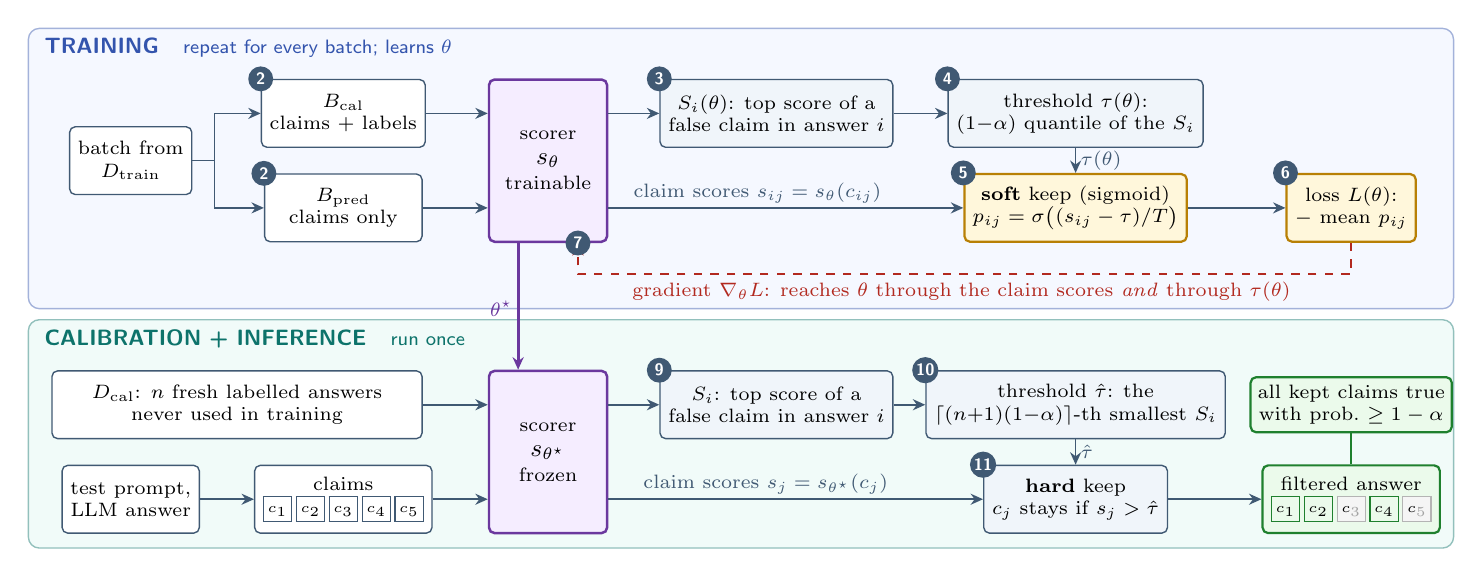
\begin{tikzpicture}[x=1cm,y=1cm,font=\scriptsize,%
  >={Stealth[length=4.5pt,width=4pt]},
  box/.style={draw=recfr,fill=white,rounded corners=2pt,align=center,inner sep=3pt,minimum height=0.86cm,line width=0.5pt},
  op/.style={box,fill=recbg},
  model/.style={box,draw=clmfr,fill=clmbg,line width=0.9pt,minimum height=2.06cm,minimum width=1.5cm},
  soft/.style={box,draw=keyfr,fill=keybg,line width=0.8pt},
  good/.style={box,draw=okfr,fill=okbg,line width=0.8pt},
  flow/.style={->,draw=recfr,line width=0.6pt},
  grad/.style={->,draw=nofr,dashed,line width=0.8pt},
  lab/.style={font=\scriptsize,text=recfr,inner sep=1.5pt},
  ttl/.style={font=\sffamily\bfseries\footnotesize,anchor=west,inner sep=0pt}]

% ================= training band =================
\node[ttl,text=thmfr] at (-0.05,0.33) {TRAINING\quad{\normalfont\sffamily\scriptsize repeat for every batch; learns $\theta$}};
\node[box] (bt) at (1.05,-1.10) {batch from\\$\Dtr$};
\node[box,minimum width=2.0cm] (bc) at (3.75,-0.50) {$\Bcal$\\claims + labels};
\node[box,minimum width=2.0cm] (bp) at (3.75,-1.70) {$\Bpred$\\claims only};
\node[model] (sc) at (6.35,-1.10) {scorer\\[1pt]{\small$s_\theta$}\\[1pt]trainable};
\node[op] (si) at (9.25,-0.50) {$S_i(\theta)$: top score of a\\false claim in answer $i$};
\node[op] (tq) at (13.05,-0.50) {threshold $\tau(\theta)$:\\$(1{-}\alpha)$ quantile of the $S_i$};
\node[soft] (sk) at (13.05,-1.70) {\textbf{soft} keep (sigmoid)\\$p_{ij}=\sigma\big((s_{ij}-\tau)/T\big)$};
\node[soft] (ls) at (16.55,-1.70) {loss $L(\theta)$:\\$-$ mean $p_{ij}$};

\draw[flow] (bt.east) -- ++(0.28,0) |- (bc.west);
\draw[flow] (bt.east) -- ++(0.28,0) |- (bp.west);
\draw[flow] (bc.east) -- (bc.east -| sc.west);
\draw[flow] (bp.east) -- (bp.east -| sc.west);
\draw[flow] (si.west -| sc.east) -- (si.west);
\draw[flow] (si.east) -- (tq.west);
\draw[flow] (tq.south) -- node[lab,right]{$\tau(\theta)$} (sk.north);
\draw[flow] (sk.west -| sc.east) -- node[lab,above,pos=0.42]{claim scores $s_{ij}=s_\theta(c_{ij})$} (sk.west);
\draw[flow] (sk.east) -- (ls.west);
\draw[grad] (ls.south) -- ++(0,-0.40) -| ($(sc.south)+(0.38,0)$);
\node[lab,text=nofr] at (11.6,-2.76) {gradient $\nabla_\theta L$: reaches $\theta$ through the claim scores \emph{and} through $\tau(\theta)$};

\node[badge] at (bc.north west) {2}; \node[badge] at (bp.north west) {2};
\node[badge] at (si.north west) {3}; \node[badge] at (tq.north west) {4};
\node[badge] at (sk.north west) {5}; \node[badge] at (ls.north west) {6};
\node[badge] at ($(sc.south)+(0.38,0.0)$) {7};

% ================= calibration + inference band =================
\node[ttl,text=deffr] at (-0.05,-3.37) {CALIBRATION + INFERENCE\quad{\normalfont\sffamily\scriptsize run once}};
\node[box,minimum width=4.7cm] (dc) at (2.40,-4.20) {$\Dcal$: $n$ fresh labelled answers\\never used in training};
\node[box] (tx) at (1.05,-5.40) {test prompt,\\LLM answer};
\node[box,minimum width=2.0cm] (tc) at (3.75,-5.40) {claims\\\cany{1}\,\cany{2}\,\cany{3}\,\cany{4}\,\cany{5}};
\node[model] (sf) at (6.35,-4.80) {scorer\\[1pt]{\small$s_{\ths}$}\\[1pt]frozen};
\node[op] (sj) at (9.25,-4.20) {$S_i$: top score of a\\false claim in answer $i$};
\node[op] (th) at (13.05,-4.20) {threshold $\tauhat$: the\\$\lceil(n{+}1)(1{-}\alpha)\rceil$-th smallest $S_i$};
\node[op] (hk) at (13.05,-5.40) {\textbf{hard} keep\\$c_j$ stays if $s_j>\tauhat$};
\node[good] (fa) at (16.55,-5.40) {filtered answer\\\ckeep{1}\,\ckeep{2}\,\cdrop{3}\,\ckeep{4}\,\cdrop{5}};
\node[good,inner sep=2.5pt,minimum height=0.7cm] (gu) at (16.55,-4.20) {all kept claims true\\with prob.\ $\ge 1-\alpha$};

\draw[flow] (dc.east) -- (dc.east -| sf.west);
\draw[flow] (tx.east) -- (tc.west);
\draw[flow] (tc.east) -- (tc.east -| sf.west);
\draw[flow] (sj.west -| sf.east) -- (sj.west);
\draw[flow] (sj.east) -- (th.west);
\draw[flow] (th.south) -- node[lab,right]{$\tauhat$} (hk.north);
\draw[flow] (hk.west -| sf.east) -- node[lab,above,pos=0.42]{claim scores $s_j=s_{\ths}(c_j)$} (hk.west);
\draw[flow] (hk.east) -- (fa.west);
\draw[okfr,line width=0.6pt] (fa.north) -- (gu.south);
\draw[->,draw=clmfr,line width=1.1pt] ($(sc.south)+(-0.38,0)$) -- node[lab,left,text=clmfr,pos=0.52]{$\ths$} ($(sf.north)+(-0.38,0)$);

\node[badge] at (sj.north west) {9}; \node[badge] at (th.north west) {10};
\node[badge] at (hk.north west) {11};

\begin{scope}[on background layer]
  \fill[thmbg!55,rounded corners=4pt] (-0.25,0.58) rectangle (17.85,-2.98);
  \draw[thmfr!45,rounded corners=4pt,line width=0.5pt] (-0.25,0.58) rectangle (17.85,-2.98);
  \fill[defbg!80,rounded corners=4pt] (-0.25,-3.12) rectangle (17.85,-6.02);
  \draw[deffr!45,rounded corners=4pt,line width=0.5pt] (-0.25,-3.12) rectangle (17.85,-6.02);
\end{scope}
\end{tikzpicture}
\end{center}
\vspace{-5pt}
{\footnotesize\textbf{Figure.} The two bands have the same shape on purpose: a training step is a small, differentiable rehearsal of inference. The differences are the yellow boxes (a sigmoid in place of the hard keep/drop rule, and a loss) and the data that sets the threshold (half a batch in training, a fresh calibration set afterwards). Numbers \lb{2}--\lb{11} refer to the lines of the algorithms below.\par}

\vspace{4pt}
\begin{minipage}[t]{0.492\linewidth}
\small
\begin{recipebox}[Algorithm 1\quad Training (learn $\theta$)]
\algin{$\Dtr$ with claim labels; error level $\alpha$; temperature $T$; step size $\eta$.}
\begin{algo}
\al \kw{repeat}
\al[1] split a random batch of $\Dtr$ into halves $\Bcal$, $\Bpred$
\al[1] \kw{for} $i\in\Bcal$:\ \ $S_i(\theta)\gets\max\limits_{j:\,y_{ij}=0}s_\theta(c_{ij})$ \cm{uses labels}
\al[1] $\tau(\theta)\gets$ the $\lceil(|\Bcal|{+}1)(1{-}\alpha)\rceil$-th smallest $S_i(\theta)$
\al[1] \kw{for} $i\in\Bpred$, all $j$:\ \ $p_{ij}\gets\sigma\big((s_\theta(c_{ij})-\tau(\theta))/T\big)$
\al[1] $L(\theta)\gets-\dfrac{1}{|\Bpred|}\sum\limits_{i\in\Bpred}\dfrac{1}{m_i}\sum\limits_{j=1}^{m_i}p_{ij}$ \cm{$-$ fraction kept}
\al[1] $\theta\gets\theta-\eta\,\nabla_\theta L(\theta)$
\al \kw{until} converged;\ \ \kw{return} $\ths$
\end{algo}
\end{recipebox}
\vspace{-10pt}
\begin{recipebox}[Algorithm 2\quad Calibration and inference ($\ths$ frozen)]
\algin{$\ths$; fresh labelled $\Dcal$ of $n$ answers; the same $\alpha$.}
\begin{algo}
\al \kw{for} $i=1,\dots,n$:\ \ $S_i\gets\max\limits_{j:\,y_{ij}=0}s_{\ths}(c_{ij})$ \cm{as line 3}
\al $\tauhat\gets$ the $\lceil(n{+}1)(1{-}\alpha)\rceil$-th smallest of $S_1,\dots,S_n$
\al \kw{for} a test answer with claims $c_1,\dots,c_m$:\\ \kw{return} $\{c_j:\ s_{\ths}(c_j)>\tauhat\}$, merged back into text
\end{algo}
\vspace{3pt}{\color{recfr!40}\hrule height 0.4pt}\vspace{4pt}
{\footnotesize\raggedright\textcolor{recfr}{\textbf{Example}} ($\alpha=0.2$, $n=9$). Sorted $S_i$: $-\infty,\,-\infty,\,0.1,\,0.2,\,0.3,\,0.4,\,0.5,\,\mathbf{0.6},\,0.8$. Since $\lceil 10\times0.8\rceil=8$, $\tauhat$ is the 8th smallest, $0.6$. A test answer with claim scores $(0.9,\,0.8,\,0.3,\,0.7,\,0.2)$ keeps $c_1,c_2,c_4$, as drawn in the figure.\par}
\end{recipebox}
\end{minipage}\hfill
\begin{minipage}[t]{0.492\linewidth}
\small
\textcolor{secblue}{\sffamily\bfseries Step by step}\par\vspace{1pt}
\begin{list}{}{\setlength{\leftmargin}{2.9em}\setlength{\labelwidth}{2.5em}\setlength{\labelsep}{0.4em}\setlength{\itemsep}{2.6pt}\setlength{\parsep}{0pt}\setlength{\topsep}{1pt}}
\item[\lb{2}] \hl{Split the batch.} One half plays the calibration set, the other plays the test answers, so the loss measures what the calibrated filter would really keep.
\item[\lb{3}] \hl{Score each answer.} After filtering, answer $i$ has no false claim left exactly when $\tau\ge S_i$, the score of its highest-scoring false claim. So $S_i$ is the smallest safe threshold for that answer ($-\infty$ if it has no false claim). Labels are used here and nowhere else.
\item[\lb{4}] \hl{Set the threshold.} The $(1{-}\alpha)$ quantile is safe for a fraction $1-\alpha$ of the half-batch. It equals one of the $S_i(\theta)$, hence one claim's score, so it is differentiable in $\theta$. A soft quantile (ConfTr, DCF) spreads the gradient over more answers.
\item[\lb{5}] \hl{Filter softly.} The rule ``keep if $s_{ij}>\tau$'' has zero gradient, so a sigmoid replaces it. $p_{ij}$ is a soft keep decision and $T$ sets how sharp it is.
\item[\lb{6}] \hl{Loss.} Minus the mean fraction of claims kept. It needs no labels: a scorer that lifts false claims also lifts $\tau$ in line~4, which removes claims everywhere. (DCF weights $p_{ij}$ by $y_{ij}$ instead.)
\item[\lb{7}] \hl{Update.} The gradient reaches $\theta$ twice: through the scores on $\Bpred$ (lift claims above the threshold) and through $\tau(\theta)$ (push the top false claims down). Together they teach the scorer to rank true claims above false ones near the threshold.
\item[\lb{9}\,\lb{10}] \hl{Recalibrate.} $\ths$ was fit to $\Dtr$, so a threshold computed there is too optimistic. $\Dcal$ is exchangeable with the test answer, which is all the guarantee needs.
\item[\lb{11}] \hl{Filter.} The hard rule, with no sigmoid and no temperature.
\end{list}
\end{minipage}

\vspace{3pt}
\begin{minipage}[t]{0.492\linewidth}
\small
\begin{okbox}[Guaranteed, for any $\ths$]
If the $n$ calibration answers and the test answer are exchangeable, then $\PP(\text{every kept claim is true})\ge 1-\alpha$. Training cannot break this: it only changes which scorer gets calibrated.
\end{okbox}
\end{minipage}\hfill
\begin{minipage}[t]{0.492\linewidth}
\small
\begin{nobox}[Not guaranteed]
How much is kept: dropping every claim is valid, so retention must be reported. Training raises it only as far as the scorer's inputs separate true from false claims. Coverage is an average over prompts, not a per-prompt promise.
\end{nobox}
\end{minipage}

\vspace{1pt}
{\scriptsize\textcolor{ourfr}{\textbf{Sources.} Filter and lines 9--11: Mohri \& Hashimoto (2024, arXiv:2402.10978). Training loop, lines 1--8: ConfTr, Stutz et al.\ (2022). Published variants with a learned claim scorer: Cherian, Gibbs \& Cand\`es (2024, \S3.3), with a prompt-dependent threshold and an exact gradient through it, and DCF (2026), for claims on a dependency graph.}\par}

\newpage
{\Large\bfseries\color{secblue} Caveats}\\[1pt]
{\small\textcolor{ourfr}{Three points that are easy to misread. For a reasoning trace, read \emph{answer} as trace, \emph{claim} as step and \emph{false} as bad.}}

\vspace{2pt}
\begin{minipage}[t]{0.492\linewidth}
\small
\cav{1}{$S_i$ looks only at the false claims}{lines 3 and 9}
The labels decide which claims are false. $S_i$ is then read off the scores of those claims, whatever the scores are. The maximum runs over the labelled false claims only, never over all claims.
\begin{blist}
\item \hl{One false claim.} $S_i$ is that claim's score, high or low. This is the usual conformal score, the score of the true label.
\item \hl{Several false claims.} The answer must still give one number, and the threshold has to remove all of them. The hardest to remove is the false claim the scorer trusts most, hence the maximum.
\item \hl{True claims never enter $S_i$,} however high they score.
\end{blist}

\vspace{5pt}
\begin{center}
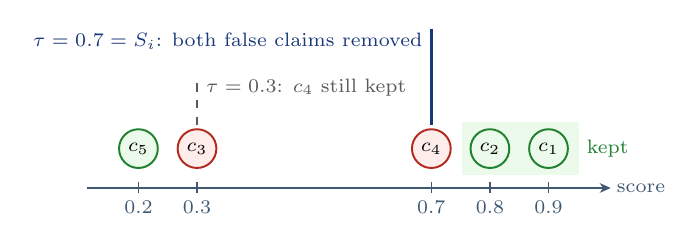
\begin{tikzpicture}[x=0.93cm,y=1cm,font=\scriptsize,
  cl/.style={circle,inner sep=0pt,minimum size=14pt,line width=0.7pt},
  tr/.style={cl,draw=okfr,fill=okbg},
  fa/.style={cl,draw=nofr,fill=nobg}]
\fill[okbg] (6.02,0.16) rectangle (7.62,0.84);
\node[anchor=west,text=okfr,inner sep=2pt] at (7.64,0.5) {kept};
\draw[recfr,line width=0.5pt,->,>={Stealth[length=4pt,width=3.5pt]}] (0.9,0) -- (8.05,0) node[right,inner sep=2pt,text=recfr]{score};
\foreach \s/\x in {0.2/1.6,0.3/2.4,0.7/5.6,0.8/6.4,0.9/7.2}{\draw[recfr,line width=0.5pt] (\x,0.07)--(\x,-0.07) node[below,inner sep=2.5pt]{\s};}
\node[tr] at (1.6,0.5) {$c_5$}; \node[fa] at (2.4,0.5) {$c_3$}; \node[fa] at (5.6,0.5) {$c_4$};
\node[tr] at (6.4,0.5) {$c_2$}; \node[tr] at (7.2,0.5) {$c_1$};
\draw[ourfr,dashed,line width=0.7pt] (2.4,0.80) -- (2.4,1.42);
\node[anchor=west,text=ourfr,inner sep=2pt] at (2.44,1.28) {$\tau=0.3$: $c_4$ still kept};
\draw[secblue,line width=0.9pt] (5.6,0.80) -- (5.6,2.02);
\node[anchor=east,text=secblue,inner sep=2pt] at (5.56,1.86) {$\tau=0.7=S_i$: both false claims removed};
\end{tikzpicture}
\end{center}
\vspace{-6pt}
{\footnotesize\textbf{Figure.} One answer with scores $(0.9,\,0.8,\,0.3,\,0.7,\,0.2)$ whose claims $c_3$ and $c_4$ are labelled false (red). A threshold of $0.3$ removes $c_3$ but keeps $c_4$. Only $\tau\ge0.7$ removes both, so $S_i=0.7$. Claim $c_1$ scores $0.9$ but is true, so it plays no part.\par}

\vspace{6pt}
\begin{oursbox}[The opposite convention]
If the scorer rates how likely a claim is to be \emph{false} (higher means more suspect), everything flips: $S_i$ is the lowest score among the false claims, and the flagged set is every claim scoring at or above the threshold.
\end{oursbox}
\end{minipage}\hfill
\begin{minipage}[t]{0.492\linewidth}
\small
\cav{2}{One score per answer, not per claim}{lines 3--4, 9--10}
\begin{blist}
\item Each answer contributes exactly one number, $S_i$, however many claims it has.
\item \hl{Why.} The guarantee is a statement about a whole answer (``every kept claim is true''), and exchangeability holds between answers. Claims inside one answer depend on each other, so pooling them as separate calibration points would break the assumption.
\item An answer with no false claim still contributes one score, $-\infty$: any threshold is safe for it.
\item Every claim needs a label to find the false ones, but only the top-scoring false claim of each answer moves the threshold.
\item \hl{Resolution.} The threshold moves in steps of $1/(n+1)$ answers. With $n=50$, as in Mohri \& Hashimoto, $\alpha$ is resolved in steps of about $2\%$, and any $\alpha<1/51$ gives $\lceil(n+1)(1-\alpha)\rceil>n$, that is $\tauhat=+\infty$: every claim is dropped.
\item \hl{In training} it is the same on $\Bcal$ (one $S_i$ per answer), while the loss on $\Bpred$ uses every claim's score.
\end{blist}

\cav{3}{The output is a subset of the original claims}{line 11}
\begin{blist}
\item Exactly the claims with $s_{\ths}(c_j)>\tauhat$, in their original order. Nothing is added, rewritten or reordered.
\item \hl{A top-scoring set.} One threshold cuts the ranked list, so the kept sets are nested: lowering $\alpha$ can only remove claims.
\item \hl{Gaps, or nothing at all.} Claim 3 may be dropped while claim 4, which relies on it, is kept. Coherent Factuality (Rubin-Toles et al., 2025) repairs this with a dependency graph.
\item \hl{The guarantee is on the set, not on rewritten text.} Mohri \& Hashimoto pass the kept claims through an LLM ``merger'' to produce prose, and that step is outside the guarantee.
\item \hl{Complement view.} The removed claims form a set that contains every false claim with probability at least $1-\alpha$, and training makes that set smaller. This is the reading that matters for failure attribution.
\end{blist}
\end{minipage}
\end{document}
